\section{Planteamiento del problema}
Ateniéndonos a los datos presentes en la Agenda del Agua 2030, en México, tan solo el 91.3\% de la población cuenta con servicio de agua potable y 89.9\% tiene cobertura de alcantarillado del cual, solo un 43.4\% recibe tratamiento. Las estimaciones esperadas rumbo a 2030 indican que se requerirá infraestructura para dar un tratamiento correcto a 7.157 miles de millones de metros cúbicos, generando una brecha de 4.3 miles de millones de metros cúbicos~\citep{aa2030}.\par
Tales objetivos se vuelven aún más alejados de convertirse en realidad cuando analizamos que, tan solo en Jalisco, de las 230 plantas de tratamiento a cargo del gobierno, para abril del 2024 solo 144 se encuentran en operación, con un tratamiento estimado de 16088 litros por segundo; y solamente una planta en construcción~\citep{CEAJ24}.\par
Así mismo, resulta alarmante el aumento de la temperatura y las constantes sequías, las cuales comprometen la seguridad hídrica de los gobiernos de cada país, la \citep{CNA2024} en su informe monitoreo de sequía advierte que, tan solo en México: 1899 de los 2471 municipios sufren de alguna de las 4 categorías diferentes de sequía, 366 condición anormalmente seca y tan solo 206 son los que no presentan algún tipo de afectación (ver figura \ref{fig:sequia}). El portal de noticias UNOTV en su artículo "¿Vacías o a tope? Ve estado actual de las presas más importantes de México tras últimas lluvias" destaca que, de las 210 presas registradas en México, solo son 180 las que almacenan el 82\% del agua destinada al sector productivo y a la población en general. De estas, solo 46 cuentan con niveles de llenado por encima del 50\%. La preocupación aumenta al pasar del tiempo, ya que a pesar presentarse lluvias durante parte de la temporada de estiaje, en la segunda quincena de junio, el nivel promedio de llenado apenas alcanza el 36\%~\citep{Cruz2024}. \par
La finalidad de este proyecto es obtener las condiciones de operación que mejor se adaptan al proceso de remoción de contaminantes con el fin de estandarizar un sistema de tratamiento eficiente y de bajo coste que pueda ser utilizado en localidades que no cuenten con un proceso de tratamiento de las aguas residuales generadas por estas, ayudando con esto a que se disminuya el número de descargas a cuerpos de agua potable, los cuales ocasionan problemas sanitarios en poblaciones que no cuentan con plantas potabilizadoras o un manejo inadecuado del recurso vital.\par
\begin{figure}[H]
	\centering
	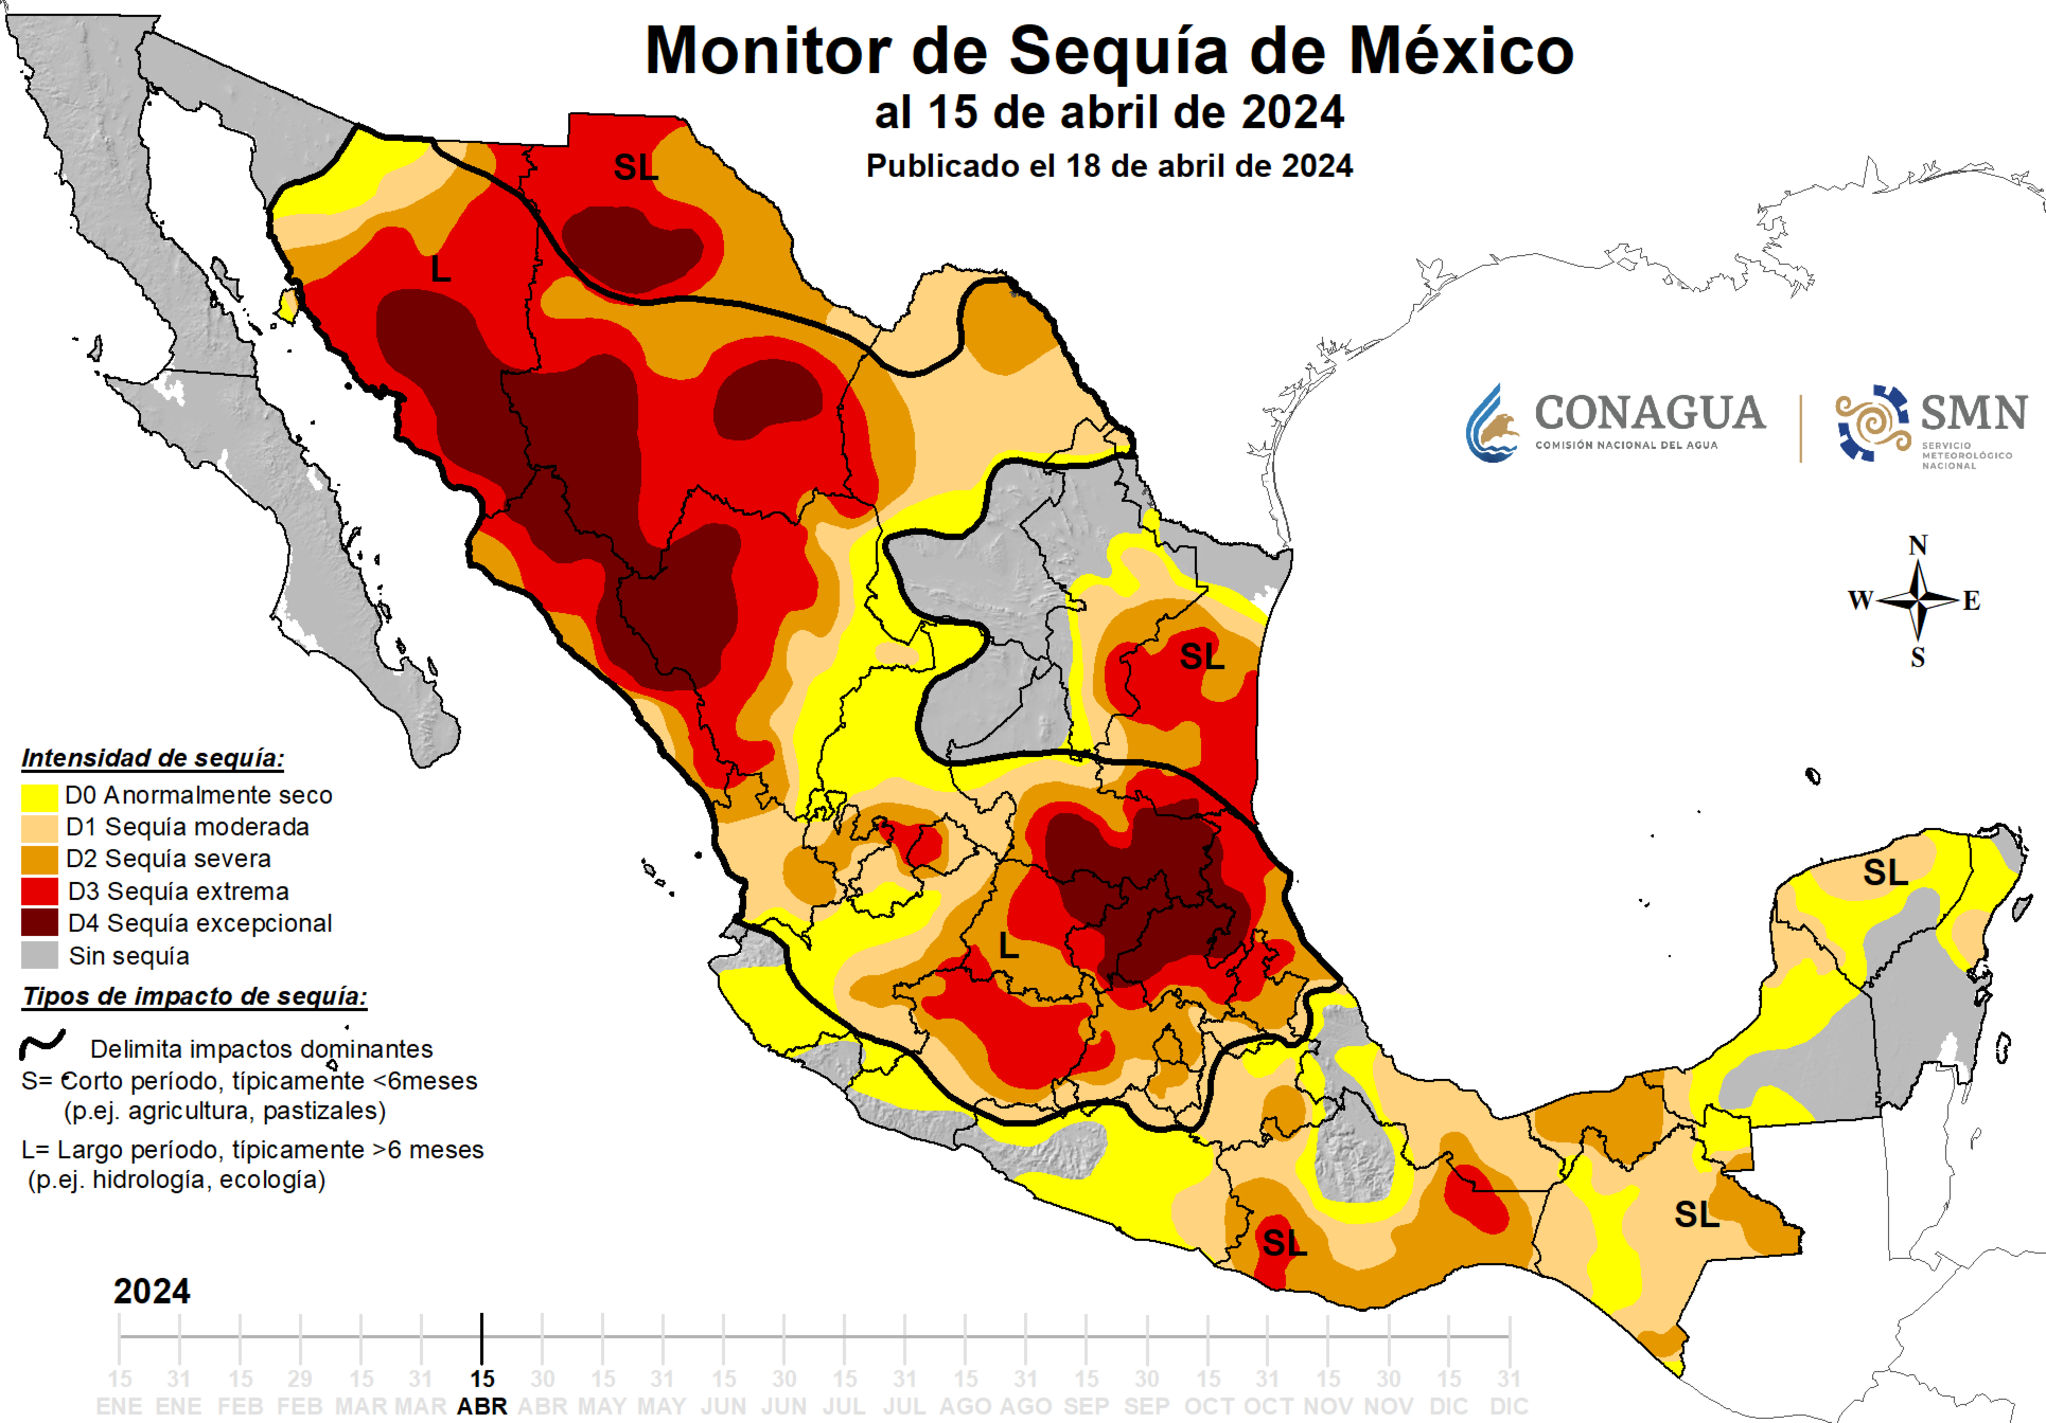
\includegraphics[scale=0.35]{../Images/Sequia.pdf}
	\\\small{Fuente: \cite{CNA2024}}
	\caption{Mapa de México dónde se muestra los niveles de sequía acorde a la intensidad al mes de abril del 2024}\label{fig:sequia}
\end{figure}
La base metodológica del proyecto toma como base los diseños de reactor y experimentos de \cite{Ramalho2003}, donde, los resultados obtenidos fueron utilizados para obtener las constantes cinéticas especificas de los lodos de la \acrshort{PTAR} municipal de Lagos de Moreno para, posteriormente desarrollar un algoritmo de MATLAB, con el cual simular las condiciones de operación del sistema de manera habitual dadas por el usuario y compararlas con las resultantes del sistema real y comparar la efectividad de predicción del algoritmo con respecto al modelo real.